\section{Distribución normal bivariante}


Decimos que un vector aleatorio $X$ sigue distrubución normal bivariante con vector de medidas $(\mu_X, \mu_Y)$, matriz de varianzas y covarianzas $\Sigma$
si tiene función de densidad conjunta

\[ f(x_1,x_2)=\frac{1}{2\pi\left| \Sigma \right|^{\frac{1}{2}}}exp\bigg{\{} \frac{-1}{2}(x_1 - \mu_1, x_2 - \mu_2)\Sigma^{-1}
\left(\begin{matrix}
    x_1 - \mu_1 \\
    x_2 - \mu_2
\end{matrix}\right) \bigg{\}}; \]
\[ \text{si}\quad \Sigma = \left( \begin{matrix}
    \sigma_1^2 & \rho\sigma_1\sigma_2 \\
    \rho\sigma_1\sigma_2 & \sigma_2^2
\end{matrix} \right) \quad \text{entonces} \qquad f(x_1,x_2)= \]
\[ = \frac{1}{2\pi\sigma_1\sigma_2\sqrt{1 - \rho^2}}exp\Biggl\{\frac{1}{2(1-\rho^2)}\left[ \left( \frac{x_1-\mu_1}{\sigma_1} \right)^2 + \left( \frac{x_2 - \mu_2}{\sigma_2} \right)^2 - 2\rho\left( \frac{x_1 - \mu_1}{\sigma_1} \right) \left( \frac{x_2 - \mu_2}{\sigma_2} \right) \right] \Biggr\} \]

\begin{figure}[htbp]
    \center
    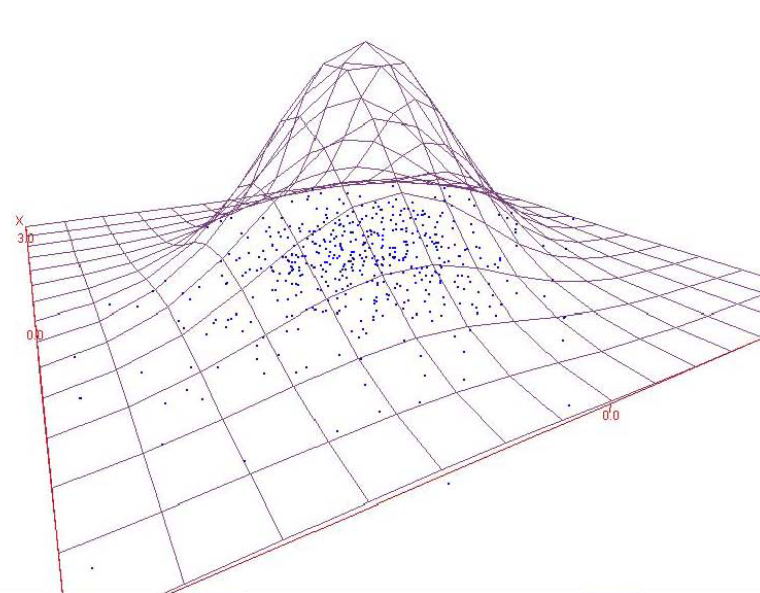
\includegraphics[scale=0.6]{img/NormalBivariante.png}
    \caption{Ejemplo de distribución normal bivariante}
\end{figure}

Las distribuciones marginales de una distribución Normal Bivariante son normales unidimensionales,

\[ X_1\thicksim N(\mu_1,\sigma_1^2) \quad \text{y} \quad X_2\thicksim N(\mu_2,\sigma_2^2) \]

donde la correlación $\rho$ controla el grado de dependencia lineal entre ellas.

\newpage

\begin{figure}[htbp]
    \center
    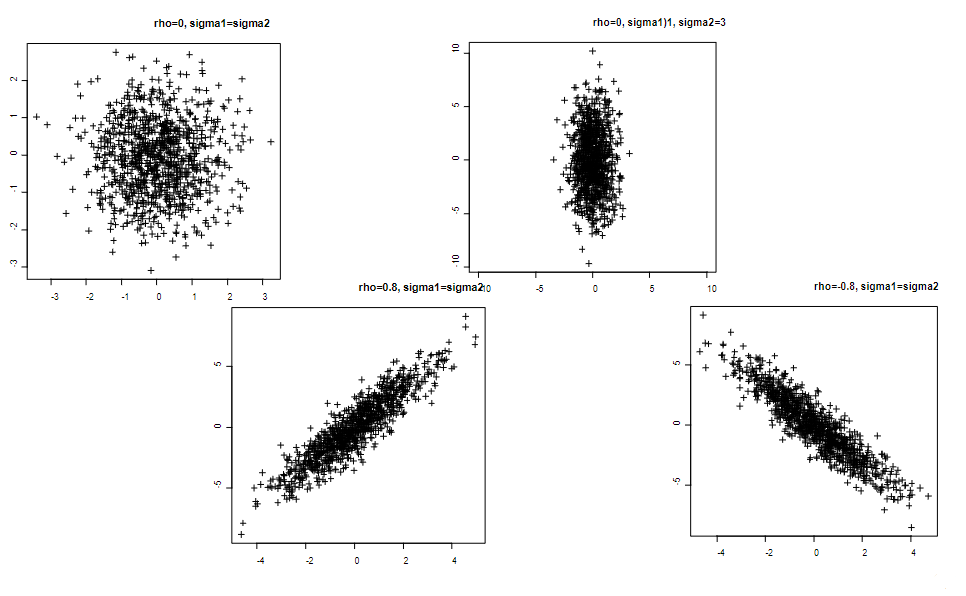
\includegraphics[scale=0.5]{img/GraficosNormalBivariable.png}
\caption{Ejemplo de distribución normal bivariante.}
\end{figure}

Las distribuciones normales bivariantes tienen las siguientes \textbf{propiedades}:
Dado $(X_1,X_2)$ un vector aleatorio normal con vector de medidas $(\mu_1,\mu_2)$ y matriz de varianzas y covarianzas $\Sigma$,
\begin{itemize}
    \item Si $\rho = 0$ entonces $X_1$ e $X_2$ son independientes
    \item Dados $a_1,a_2,a_3 \in \mathbb{R}$, $a_1X_1 + a_2X_2 + a_3$ es normal
    \item $X_1 \bigg{/} X_2 = x_2$ es normal y $X_2 \bigg{/} X_1 = x_1$ es normal
    \item Sea $A \in \mathcal{M}_{2\times2}$, $X$ vector aleatorio de dimensión 2, $X\thicksim N(\mu_X, \Sigma_X)$ entonces \\ $Y=AX\thicksim N(\mu_Y, \Sigma_Y)$ donde $\mu_Y = A\mu_X$ y $\Sigma_Y = A\Sigma_XA^t$
\end{itemize}

Dado $(X, Y)$ un vector aleatorio normal con medidas $(\mu_X, \mu_Y)$ y matriz de varianzas y covarianzas $\Sigma$

\[ Y \bigg{/} X = x \thicksim N(\mu_2 + \rho(\frac{\sigma_2}{\sigma_1})(x-\mu_1), \sigma_2^2(1-\rho^2)) \]
